\documentclass[11pt]{report}

\usepackage{hyperref}
\usepackage{amsmath}
\usepackage{pgfplots}

\title{\textbf{{\Large Solving sudoku using a backtracking algorithm}}}
\author{Dlamini Christopher(1965919).~Hlomuka Siyabonga().~Musara Walter(1830229)}
\begin{document}
\maketitle
    \section{Aim}
        Given our implementation of a sudoku solving algorithm , that makes use of backtracking, we want to empirically analyse 
        the perfomance of the said algorithm.Next we will compare the empirical analysis's results to the theory and see how our algorithm fares against
        a bruteforce approach. We assume all input boards are 9x9.

    \section{Summary of theory}
        \subsection{sudoku}
            \hyperref[sec:wikiwand]{1} defines Sudoku as a logic-based, combinatorial number-placement puzzle. In classic sudoku, the objective is
            to fill a 9x9 grid with digits so that each column, each row, and each of the nine 3x3 subgrids that
            compose the grid (also called "boxes", "blocks", or "regions") contain all of the digits from 1 to 9.
            The puzzle setter provides a partially completed grid, which for a well-posed puzzle has a single
            solution.             

        \subsection{Backtracking algorithm}
            The obvious way for a computer to solve it is using a bruteforce method. This ,of course, is impractical so smarter algorithms are 
            needed. One such algorithm is one that uses backtracking.\\

            A backtracking algorithm for soduku recursively attempts to solve a given soduku
            puzzle by testing all possible configurations towards a solution until a solution is found.Unlike a bruteforce approach, each time a
            configuration is tested, if a solution is not found, the algorithm backtracks to test another possible
            configuration. This goes on till a solution is found or all configurations have been exhausted.

        \subsection{Perfomance of backtracking algorithm}
            For every unassigned index, there are 9 possible options so the time complexity is \begin{equation}O(9^{n^2}) \label{sec:comp}\end{equation} 
            The time complexity remains the same but there will be some early pruning so the time taken will be
            much less than the naive algorithm but the upper bound time complexity remains the same.

    \section{Experimental Methodology}
        The algorithm is implemented in java.To measure the perfomance we record the current time right
        before the algorithm starts solving a puzzle and then right after. This will indicate the approximate time it took to solve the
        sudoku puzzle. There will be different sudoku puzzle inputs.These puzzles will differ in the level of
        difficulty and all their solve-times will be recorded. We will also count the number of operations on the different puzzles. 
        All of these results  will be aid us in coming to a decisive conclusion after analysis.

    \section{Results}
        \subsection{Some sample inputs with their solve-times}
            \begin{table}[h!]
                \begin{center}
                    \caption{Sample inputs and their results}
                    \begin{tabular}{l|r|r}
                        \textbf{input} & \textbf{time(ns)} & \textbf{operations}\\
                        \hline
                        
                        %-------------------
                        \hyperref[sec:easy0]{easy 0} & 712796 & 82\\
                        \hyperref[sec:easy1]{easy 1} & 644607 & 82\\

                        \hyperref[sec:mid0]{medium 0} & 834085 & 178\\
                        \hyperref[sec:mid1]{medium 1} & 1100161 & 503\\

                        \hyperref[sec:hard0]{hard 0} & 6623904 & 9741\\
                        \hyperref[sec:hard1]{hard 1} & 12554631 & 27694\\

                        \hyperref[sec:vhard0]{very hard 0} & 13851059 & 27040\\
                        \hyperref[sec:vhard1]{very hard 1} & 7422293 & 11355\\

                        solved puzzle & 169714 & 82\\
                        empty puzzle & 1087386 & 392\\

                        \hyperref[sec:miss]{missing 1 value} & 187842 & 82\\ 

                     
                    \end{tabular}
                \end{center}
            \end{table}
        Taking the puzzle inputs with the longest durations from each difficulty level produces the following graph checking concurrency:\\

        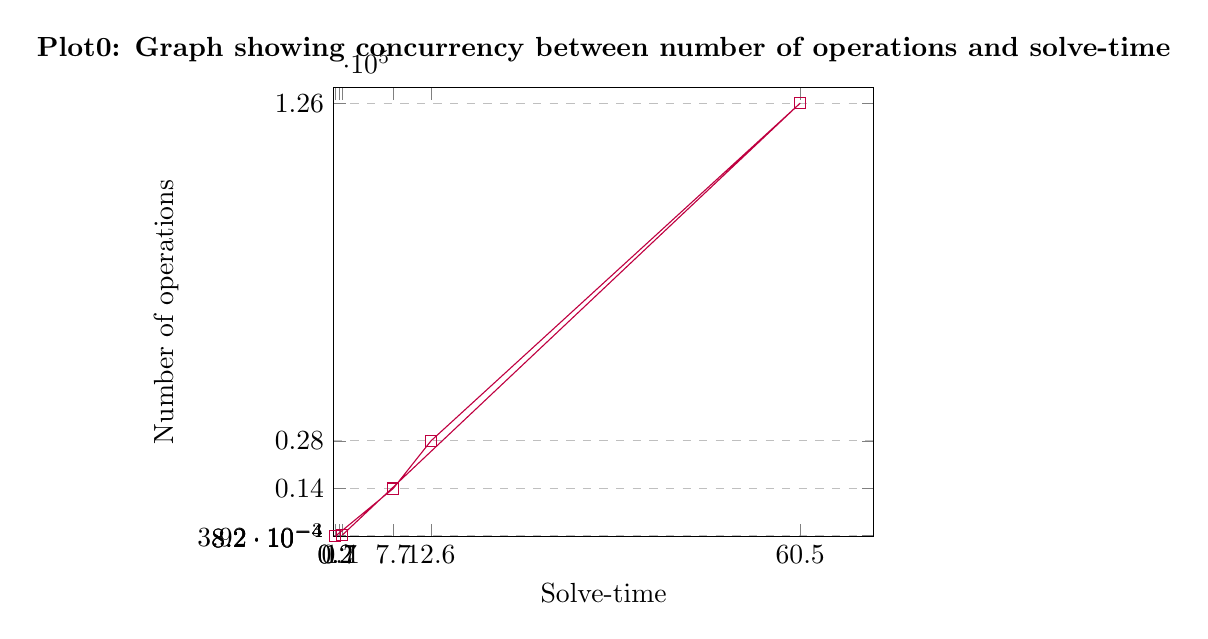
\begin{tikzpicture}
        \begin{axis}[
            title={\textbf{Plot0: Graph showing concurrency between number of operations and solve-time}},
            xlabel={Solve-time},
            ylabel={Number of operations},
            xmin=0, xmax=70,
            ymin=80, ymax=130000,
            xtick={0.2,0.2,0.7,1.1,7.7,12.6,60.5},
            %xtick={169714,187842,712796,1087386,7720505,12554631,60450250},
            ytick={82,82,82,392,13884,27694,125574},
            ymajorgrids=true,
            grid style=dashed,
        ]

        \addplot[
            color=purple,
            mark=square,
            ]
            coordinates {
            (0.2 ,82)(7.7 ,13884)(12.6 ,27694)(60.5 ,125574)(1.1 ,392)
            };
            
        \end{axis}
        \end{tikzpicture}\\

        Now we check the perfomances with respect to the level of  difficulty:\\

        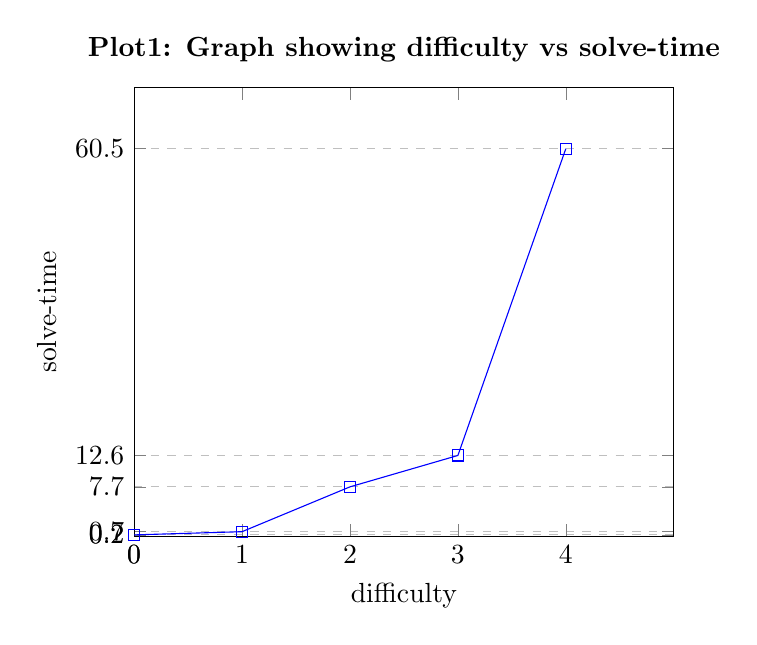
\begin{tikzpicture}
        \begin{axis}[
            title=\textbf{{Plot1: Graph showing difficulty vs solve-time}},
            xlabel={difficulty},
            ylabel={solve-time},
            xmin=0, xmax=5,
            ymin=0, ymax=70,
            xtick={0, 0, 1, 2,3,4},
            ytick={0.2,0.2,0.7,7.7,12.6,60.5},
            %xtick={169714,187842,712796,7720505,12554631,60450250},
            ymajorgrids=true,
            grid style=dashed,
        ]

        \addplot[
            color=blue,
            mark=square,
            ]
            coordinates {
            (0,0.2)(1,0.7)(2,7.7)(3,12.6)(4,60.5)
            };
            
        \end{axis}
        \end{tikzpicture}\\


        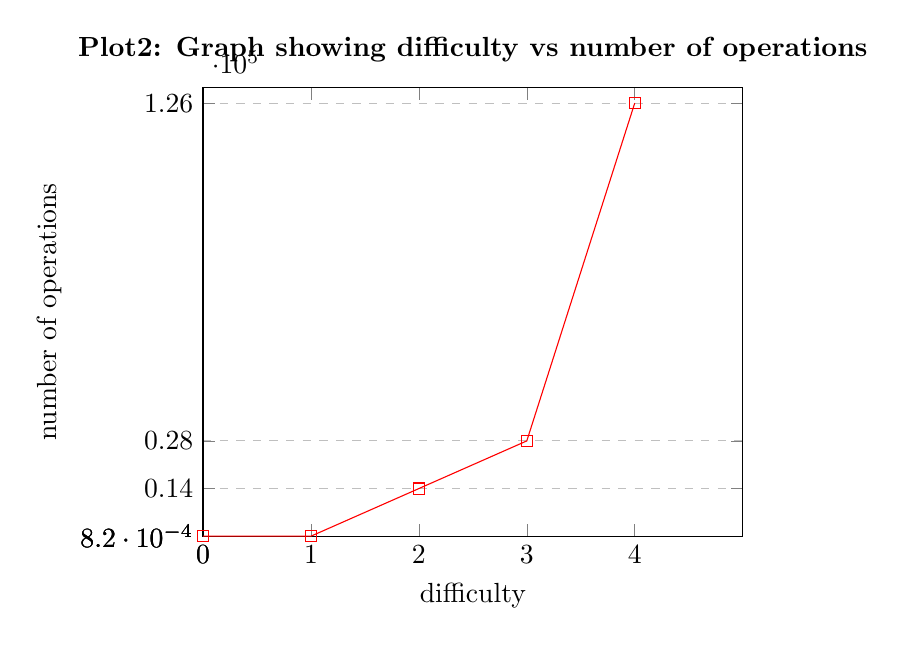
\begin{tikzpicture}
        \begin{axis}[
            title=\textbf{{Plot2: Graph showing difficulty vs number of operations}},
            xlabel={difficulty},
            ylabel={number of operations},
            xmin=0, xmax=5,
            ymin=80, ymax=130000,
            xtick={0, 0, 1, 2,3,4},
            ytick={82,82,82,13884,27694,125574},
            ymajorgrids=true,
            grid style=dashed,
        ]

        \addplot[
            color=red,
            mark=square,
            ]
            coordinates {
            (0,82)(1,82)(2,13884)(3,27694)(4,125574)
            };
            
        \end{axis}
        \end{tikzpicture} 

    \section{Interpretation of results}
        The table and the 3 plots above show some reassuring trends:\\
        \begin{itemize}
            \item There is a strong positive correlation between the solve-time and the number of operations as seen in Plot0.
            \item The solve time is directly proportional to the level of difficulty. Plot1 shows this.
            \item As expected given the first 2 statements, the number of operations the algorithm does is also directly proportional
             to the level of difficulty. This is confirmed in Plot2.
        \end{itemize}

    \section{Relating the results to the theory}
        The theoratical complexity is given by \(O(9^{n^2})\), in this case being \(1.97*10^{77}\).This is confirmed by
        the results as no number of operations to solve single sudoku puzzle reached \(1.97*10^{77}\), thus the
        equivalent time of \(1.97*10^{77}\) operations will not be reached due to the strong positive correlation
        between operations and time to solve puzzle.

    \section{conclusion}
        Solving Sudoku using a backtracking algorithm method, like our algorithm, means trying each
        available number across all empty cells. Such an algorithm has a runtime complexity of
        \(O(9^{n^2})\), where n is size of the Sudoku puzzle. The algorithm performs \(1.97*10^{77}\)
        operations to find a solution. That is impractical, however in practice the runtime varies according to
        the difficulty of the puzzle itself and the number of options for each empty cell ,as our results have shown. Therefore the time
        complexity of \(O(9^{n^2})\) is valid for the backtracking algorithm as it is just the upper bound. Our algorithm will have a 
        better perfomance than the bruteforce approach.             

    \section{Sample inputs}
        \subsection{easy 0} \label{sec:easy0}
            0 0 3 0 0 4 0 1 6\\ 
            0 7 4 9 0 0 0 0 0\\
            0 0 8 5 3 0 0 4 0\\
            0 6 2 0 0 0 4 0 0\\
            0 0 0 0 0 2 3 6 8\\
            4 0 0 8 1 0 0 0 0\\
            0 0 0 6 0 8 0 0 7\\
            7 2 0 0 9 0 0 0 0\\
            5 8 0 7 0 0 6 9 0\\

        
        \subsection{easy 1} \label{sec:easy1}
            3 7 0 9 0 0 2 8 0\\
            0 0 1 2 5 0 0 0 0\\
            0 0 0 0 0 0 9 0 0\\
            5 8 2 0 4 0 7 0 0\\
            0 0 0 0 8 0 5 9 0\\
            0 0 0 7 0 5 0 4 0\\
            0 0 6 0 0 2 0 7 3\\
            4 0 3 1 6 7 8 0 0\\
            0 5 0 0 0 0 0 6 0\\

        \subsection{medium 0} \label{sec:mid0}
            7 0 0 8 0 0 9 0 3\\
            0 0 0 2 0 0 0 1 8\\
            0 0 1 0 0 3 0 0 0\\
            0 1 5 0 0 0 3 4 0\\
            2 0 0 0 0 8 6 0 1\\
            0 0 3 0 7 4 0 0 0\\
            0 0 6 3 0 0 0 8 0\\
            0 3 0 0 0 5 1 0 9\\
            9 5 0 0 8 0 0 0 0\\    

        \subsection{medium 1} \label{sec:mid1}
            5 0 7 0 0 9 0 0 0\\
            0 4 0 0 0 5 0 9 2\\
            0 0 2 0 0 0 3 5 0\\
            0 0 0 0 9 0 8 4 1\\
            0 1 4 0 8 0 0 0 0\\
            2 8 0 7 1 0 0 0 0\\
            0 0 0 9 6 0 0 8 0\\
            0 2 5 0 0 0 0 0 9\\
            3 0 0 0 0 8 7 0 0\\

       \subsection{hard 0} \label{sec:hard0}
            0 5 3 0 6 0 0 0 0\\
            0 0 0 0 0 3 0 2 6\\
            2 9 0 0 0 8 5 0 0\\
            0 0 2 1 0 0 0 3 0\\
            0 7 5 0 0 0 0 0 0\\
            0 0 0 0 0 2 8 0 1\\
            3 0 0 9 0 0 0 0 0\\
            5 0 1 0 4 0 9 0 2\\
            0 0 0 0 0 0 3 7 0\\

        \subsection{hard 1} \label{sec:hard1}    
            0 0 0 0 4 0 0 3 0\\
            0 0 0 1 0 7 0 6 0\\
            1 0 0 0 0 0 0 4 5\\
            6 0 0 0 0 8 0 7 0\\
            0 7 0 9 6 3 0 5 0\\
            0 1 0 4 0 0 0 0 9\\
            4 8 0 0 0 0 0 0 3\\
            0 9 0 6 0 1 0 0 0\\
            0 5 0 0 3 0 0 0 0\\

        \subsection{very hard 0} \label{sec:vhard0}
            0 0 6 0 5 0 0 7 3\\
            0 3 0 2 0 0 0 0 8\\
            0 0 0 1 3 0 0 0 0\\
            0 0 9 0 0 0 2 0 0\\
            0 2 0 0 1 0 0 3 0\\
            0 0 7 0 0 0 9 0 0\\
            0 0 0 0 6 8 0 0 0\\
            4 0 0 0 0 1 0 5 0\\
            5 1 0 0 4 0 3 0 0\\

        \subsection{very hard 1} \label{sec:vhard1}
            0 8 4 0 0 0 0 0 0\\
            0 0 9 0 3 0 8 0 0\\
            7 0 0 0 0 2 1 0 0\\
            0 7 0 0 0 0 0 0 1\\
            0 0 8 4 0 1 0 0 0\\
            0 0 0 3 5 0 0 6 0\\
            0 5 0 6 0 0 0 0 0\\
            1 0 0 0 0 0 3 0 8\\
            4 0 7 0 0 0 0 9 0\\

        \subsection{missing 1 value} \label{sec:miss}
            1 2 3 4 5 6 7 8 0\\
            4 5 6 7 8 9 1 2 3\\
            7 8 9 1 2 3 4 5 6\\
            2 1 4 3 6 5 8 9 7\\
            3 6 5 8 9 7 2 1 4\\
            8 9 7 2 1 4 3 6 5\\
            5 3 1 6 4 2 9 7 8\\
            6 4 2 9 7 8 5 3 1\\
            9 7 8 5 3 1 6 4 2\\
        
    \section{References}
        [1] https://www.wikiwand.com/en/Sudoku \label{sec:wikiwand}\\
            https://www.101computing.net/backtracking-algorithm-sudoku-solver/ \\
            https://en.wikipedia.org/wiki/Sudoku\\
            https://www.geeksforgeeks.org/sudoku-backtracking-7/ \\
            https://medium.com/optima-blog/solving-sudoku-fast-702912c13307 \\
\end{document}    